


% Header, overrides base

    % Make sure that the sphinx doc style knows who it inherits from.
    \def\sphinxdocclass{article}

    % Declare the document class
    \documentclass[letterpaper,10pt,english]{/usr/share/sphinx/texinputs/sphinxhowto}

    % Imports
    \usepackage[utf8]{inputenc}
    \DeclareUnicodeCharacter{00A0}{\\nobreakspace}
    \usepackage[T1]{fontenc}
    \usepackage{babel}
    \usepackage{times}
    \usepackage{import}
    \usepackage[Bjarne]{/usr/share/sphinx/texinputs/fncychap}
    \usepackage{longtable}
    \usepackage{/usr/share/sphinx/texinputs/sphinx}
    \usepackage{multirow}

    \usepackage{amsmath}
    \usepackage{amssymb}
    \usepackage{ucs}
    \usepackage{enumerate}

    % Used to make the Input/Output rules follow around the contents.
    \usepackage{needspace}

    % Pygments requirements
    \usepackage{fancyvrb}
    \usepackage{color}
    % ansi colors additions
    \definecolor{darkgreen}{rgb}{.12,.54,.11}
    \definecolor{lightgray}{gray}{.95}
    \definecolor{brown}{rgb}{0.54,0.27,0.07}
    \definecolor{purple}{rgb}{0.5,0.0,0.5}
    \definecolor{darkgray}{gray}{0.25}
    \definecolor{lightred}{rgb}{1.0,0.39,0.28}
    \definecolor{lightgreen}{rgb}{0.48,0.99,0.0}
    \definecolor{lightblue}{rgb}{0.53,0.81,0.92}
    \definecolor{lightpurple}{rgb}{0.87,0.63,0.87}
    \definecolor{lightcyan}{rgb}{0.5,1.0,0.83}

    % Needed to box output/input
    \usepackage{tikz}
        \usetikzlibrary{calc,arrows,shadows}
    \usepackage[framemethod=tikz]{mdframed}

    \usepackage{alltt}

    % Used to load and display graphics
    \usepackage{graphicx}
    \graphicspath{ {figs/} }
    \usepackage[Export]{adjustbox} % To resize

    % used so that images for notebooks which have spaces in the name can still be included
    \usepackage{grffile}


    % For formatting output while also word wrapping.
    \usepackage{listings}
    \lstset{breaklines=true}
    \lstset{basicstyle=\small\ttfamily}
    \def\smaller{\fontsize{9.5pt}{9.5pt}\selectfont}

    %Pygments definitions
    
\makeatletter
\def\PY@reset{\let\PY@it=\relax \let\PY@bf=\relax%
    \let\PY@ul=\relax \let\PY@tc=\relax%
    \let\PY@bc=\relax \let\PY@ff=\relax}
\def\PY@tok#1{\csname PY@tok@#1\endcsname}
\def\PY@toks#1+{\ifx\relax#1\empty\else%
    \PY@tok{#1}\expandafter\PY@toks\fi}
\def\PY@do#1{\PY@bc{\PY@tc{\PY@ul{%
    \PY@it{\PY@bf{\PY@ff{#1}}}}}}}
\def\PY#1#2{\PY@reset\PY@toks#1+\relax+\PY@do{#2}}

\def\PY@tok@gd{\def\PY@tc##1{\textcolor[rgb]{0.63,0.00,0.00}{##1}}}
\def\PY@tok@gu{\let\PY@bf=\textbf\def\PY@tc##1{\textcolor[rgb]{0.50,0.00,0.50}{##1}}}
\def\PY@tok@gt{\def\PY@tc##1{\textcolor[rgb]{0.00,0.25,0.82}{##1}}}
\def\PY@tok@gs{\let\PY@bf=\textbf}
\def\PY@tok@gr{\def\PY@tc##1{\textcolor[rgb]{1.00,0.00,0.00}{##1}}}
\def\PY@tok@cm{\let\PY@it=\textit\def\PY@tc##1{\textcolor[rgb]{0.25,0.50,0.50}{##1}}}
\def\PY@tok@vg{\def\PY@tc##1{\textcolor[rgb]{0.10,0.09,0.49}{##1}}}
\def\PY@tok@m{\def\PY@tc##1{\textcolor[rgb]{0.40,0.40,0.40}{##1}}}
\def\PY@tok@mh{\def\PY@tc##1{\textcolor[rgb]{0.40,0.40,0.40}{##1}}}
\def\PY@tok@go{\def\PY@tc##1{\textcolor[rgb]{0.50,0.50,0.50}{##1}}}
\def\PY@tok@ge{\let\PY@it=\textit}
\def\PY@tok@vc{\def\PY@tc##1{\textcolor[rgb]{0.10,0.09,0.49}{##1}}}
\def\PY@tok@il{\def\PY@tc##1{\textcolor[rgb]{0.40,0.40,0.40}{##1}}}
\def\PY@tok@cs{\let\PY@it=\textit\def\PY@tc##1{\textcolor[rgb]{0.25,0.50,0.50}{##1}}}
\def\PY@tok@cp{\def\PY@tc##1{\textcolor[rgb]{0.74,0.48,0.00}{##1}}}
\def\PY@tok@gi{\def\PY@tc##1{\textcolor[rgb]{0.00,0.63,0.00}{##1}}}
\def\PY@tok@gh{\let\PY@bf=\textbf\def\PY@tc##1{\textcolor[rgb]{0.00,0.00,0.50}{##1}}}
\def\PY@tok@ni{\let\PY@bf=\textbf\def\PY@tc##1{\textcolor[rgb]{0.60,0.60,0.60}{##1}}}
\def\PY@tok@nl{\def\PY@tc##1{\textcolor[rgb]{0.63,0.63,0.00}{##1}}}
\def\PY@tok@nn{\let\PY@bf=\textbf\def\PY@tc##1{\textcolor[rgb]{0.00,0.00,1.00}{##1}}}
\def\PY@tok@no{\def\PY@tc##1{\textcolor[rgb]{0.53,0.00,0.00}{##1}}}
\def\PY@tok@na{\def\PY@tc##1{\textcolor[rgb]{0.49,0.56,0.16}{##1}}}
\def\PY@tok@nb{\def\PY@tc##1{\textcolor[rgb]{0.00,0.50,0.00}{##1}}}
\def\PY@tok@nc{\let\PY@bf=\textbf\def\PY@tc##1{\textcolor[rgb]{0.00,0.00,1.00}{##1}}}
\def\PY@tok@nd{\def\PY@tc##1{\textcolor[rgb]{0.67,0.13,1.00}{##1}}}
\def\PY@tok@ne{\let\PY@bf=\textbf\def\PY@tc##1{\textcolor[rgb]{0.82,0.25,0.23}{##1}}}
\def\PY@tok@nf{\def\PY@tc##1{\textcolor[rgb]{0.00,0.00,1.00}{##1}}}
\def\PY@tok@si{\let\PY@bf=\textbf\def\PY@tc##1{\textcolor[rgb]{0.73,0.40,0.53}{##1}}}
\def\PY@tok@s2{\def\PY@tc##1{\textcolor[rgb]{0.73,0.13,0.13}{##1}}}
\def\PY@tok@vi{\def\PY@tc##1{\textcolor[rgb]{0.10,0.09,0.49}{##1}}}
\def\PY@tok@nt{\let\PY@bf=\textbf\def\PY@tc##1{\textcolor[rgb]{0.00,0.50,0.00}{##1}}}
\def\PY@tok@nv{\def\PY@tc##1{\textcolor[rgb]{0.10,0.09,0.49}{##1}}}
\def\PY@tok@s1{\def\PY@tc##1{\textcolor[rgb]{0.73,0.13,0.13}{##1}}}
\def\PY@tok@sh{\def\PY@tc##1{\textcolor[rgb]{0.73,0.13,0.13}{##1}}}
\def\PY@tok@sc{\def\PY@tc##1{\textcolor[rgb]{0.73,0.13,0.13}{##1}}}
\def\PY@tok@sx{\def\PY@tc##1{\textcolor[rgb]{0.00,0.50,0.00}{##1}}}
\def\PY@tok@bp{\def\PY@tc##1{\textcolor[rgb]{0.00,0.50,0.00}{##1}}}
\def\PY@tok@c1{\let\PY@it=\textit\def\PY@tc##1{\textcolor[rgb]{0.25,0.50,0.50}{##1}}}
\def\PY@tok@kc{\let\PY@bf=\textbf\def\PY@tc##1{\textcolor[rgb]{0.00,0.50,0.00}{##1}}}
\def\PY@tok@c{\let\PY@it=\textit\def\PY@tc##1{\textcolor[rgb]{0.25,0.50,0.50}{##1}}}
\def\PY@tok@mf{\def\PY@tc##1{\textcolor[rgb]{0.40,0.40,0.40}{##1}}}
\def\PY@tok@err{\def\PY@bc##1{\fcolorbox[rgb]{1.00,0.00,0.00}{1,1,1}{##1}}}
\def\PY@tok@kd{\let\PY@bf=\textbf\def\PY@tc##1{\textcolor[rgb]{0.00,0.50,0.00}{##1}}}
\def\PY@tok@ss{\def\PY@tc##1{\textcolor[rgb]{0.10,0.09,0.49}{##1}}}
\def\PY@tok@sr{\def\PY@tc##1{\textcolor[rgb]{0.73,0.40,0.53}{##1}}}
\def\PY@tok@mo{\def\PY@tc##1{\textcolor[rgb]{0.40,0.40,0.40}{##1}}}
\def\PY@tok@kn{\let\PY@bf=\textbf\def\PY@tc##1{\textcolor[rgb]{0.00,0.50,0.00}{##1}}}
\def\PY@tok@mi{\def\PY@tc##1{\textcolor[rgb]{0.40,0.40,0.40}{##1}}}
\def\PY@tok@gp{\let\PY@bf=\textbf\def\PY@tc##1{\textcolor[rgb]{0.00,0.00,0.50}{##1}}}
\def\PY@tok@o{\def\PY@tc##1{\textcolor[rgb]{0.40,0.40,0.40}{##1}}}
\def\PY@tok@kr{\let\PY@bf=\textbf\def\PY@tc##1{\textcolor[rgb]{0.00,0.50,0.00}{##1}}}
\def\PY@tok@s{\def\PY@tc##1{\textcolor[rgb]{0.73,0.13,0.13}{##1}}}
\def\PY@tok@kp{\def\PY@tc##1{\textcolor[rgb]{0.00,0.50,0.00}{##1}}}
\def\PY@tok@w{\def\PY@tc##1{\textcolor[rgb]{0.73,0.73,0.73}{##1}}}
\def\PY@tok@kt{\def\PY@tc##1{\textcolor[rgb]{0.69,0.00,0.25}{##1}}}
\def\PY@tok@ow{\let\PY@bf=\textbf\def\PY@tc##1{\textcolor[rgb]{0.67,0.13,1.00}{##1}}}
\def\PY@tok@sb{\def\PY@tc##1{\textcolor[rgb]{0.73,0.13,0.13}{##1}}}
\def\PY@tok@k{\let\PY@bf=\textbf\def\PY@tc##1{\textcolor[rgb]{0.00,0.50,0.00}{##1}}}
\def\PY@tok@se{\let\PY@bf=\textbf\def\PY@tc##1{\textcolor[rgb]{0.73,0.40,0.13}{##1}}}
\def\PY@tok@sd{\let\PY@it=\textit\def\PY@tc##1{\textcolor[rgb]{0.73,0.13,0.13}{##1}}}

\def\PYZbs{\char`\\}
\def\PYZus{\char`\_}
\def\PYZob{\char`\{}
\def\PYZcb{\char`\}}
\def\PYZca{\char`\^}
\def\PYZsh{\char`\#}
\def\PYZpc{\char`\%}
\def\PYZdl{\char`\$}
\def\PYZti{\char`\~}
% for compatibility with earlier versions
\def\PYZat{@}
\def\PYZlb{[}
\def\PYZrb{]}
\makeatother


    %Set pygments styles if needed...
    
        \definecolor{nbframe-border}{rgb}{0.867,0.867,0.867}
        \definecolor{nbframe-bg}{rgb}{0.969,0.969,0.969}
        \definecolor{nbframe-in-prompt}{rgb}{0.0,0.0,0.502}
        \definecolor{nbframe-out-prompt}{rgb}{0.545,0.0,0.0}

        \newenvironment{ColorVerbatim}
        {\begin{mdframed}[%
            roundcorner=1.0pt, %
            backgroundcolor=nbframe-bg, %
            userdefinedwidth=1\linewidth, %
            leftmargin=0.1\linewidth, %
            innerleftmargin=0pt, %
            innerrightmargin=0pt, %
            linecolor=nbframe-border, %
            linewidth=1pt, %
            usetwoside=false, %
            everyline=true, %
            innerlinewidth=3pt, %
            innerlinecolor=nbframe-bg, %
            middlelinewidth=1pt, %
            middlelinecolor=nbframe-bg, %
            outerlinewidth=0.5pt, %
            outerlinecolor=nbframe-border, %
            needspace=0pt
        ]}
        {\end{mdframed}}
        
        \newenvironment{InvisibleVerbatim}
        {\begin{mdframed}[leftmargin=0.1\linewidth,innerleftmargin=3pt,innerrightmargin=3pt, userdefinedwidth=1\linewidth, linewidth=0pt, linecolor=white, usetwoside=false]}
        {\end{mdframed}}

        \renewenvironment{Verbatim}[1][\unskip]
        {\begin{alltt}\smaller}
        {\end{alltt}}
    

    % Help prevent overflowing lines due to urls and other hard-to-break 
    % entities.  This doesn't catch everything...
    \sloppy

    % Document level variables
    \title{StarCraft 2: An Analysis of Player Ranking}
    \date{May 9, 2014}
    \release{}
    \author{James Bladen and Steven Chang}
    \renewcommand{\releasename}{}

    % TODO: Add option for the user to specify a logo for his/her export.
    \newcommand{\sphinxlogo}{}

    % Make the index page of the document.
    \makeindex

    % Import sphinx document type specifics.
     


% Body

    % Start of the document
    \begin{document}

        
            \maketitle
        

        


        
        \part{Introduction}Source code and data may be found at github.com/stchang22/Stat222

StarCraft 2 is a one-on-one real-time strategy game where players gather
resources to build up armies and go defeat their opponents' armies. When
playing online against other people, players are classified into one of
six possible leagues based on their wins and losses: Bronze (the
lowest), Silver, Gold, Platinum, Diamond, and Master (the highest).

This project aims to focus on this classification aspect of StarCraft 2
(referred to as SC2 from here on out). There are two goals for the
project: to determine which skills help set players apart from one
another, and to predict a league for a new player. Casual players often
want to know how skilled they are without having to spend the time to
play enough games for an accurate representation of their skill level.
Hopefully, this project will give these players a better idea of their
skill without the drawbacks of the ranking system that is currently in
place.

The current ranking is based off Arpod Elo's rating system that was
originally created as a way to improve chess rating system. This method
has been adopted by many sports and games. The basic idea of the rating
system is that you are assigned a numeric value for your rating, and
when playing against other players your rating goes up or down based on
whether you win or lose. When playing against a player with a higher
rating, you are able to win more points than when you play against an
opponent with a less rating. The general idea is that if you are playing
against a `better' opponent you should be able to win more, and should
not be punished as hard when you lose. In SC2 they assign leagues based
off of your current ELO rating, essentially binning them into 6
categories for each of the 6 leagues.

There are some drawbacks that come along with this particular rating
system, which this project is going to try to find solutions for. There
are three main problems that occur in the implementation for SC2. First,
it takes many games in order for your rating points to accurately match
your skill level. In the short term, there is a lot of variability in
your rating so it is hard to use it as a reliable measure of your skill.
Secondly, if you happen to have a rating that is higher than your actual
skill level, the system encourages you to stop playing in order to
protect your rating. Because the ranking is based purely off wins and
losses, if you stop playing your ranking will stay the same. The last
problem with the ranking is that due to inflation of points, it is
difficult to use it to compare your skill to somebody from a previous
time period. The ranking is what is called a zero sum game. When someone
gains points, someone else loses that many points. So with more people
playing the game, there are more points available and thus point
inflation happens. Deflation can happen due to players joining the
leagues as new players and leaving once they have already gotten many
points. Very good players who stop playing will take away many points
from the overall pool of players, never to be seen again. Thus, when
comparing your rating with someone from a different time period, you
have no idea what your point value truly means compared to a point value
from a different time period.

Our goal in this project is to come up with a way of determining player
skill that circumvents these issues. Ideally, we want to find some
variables that account for actual player skill better than relying on
wins and losses. That way we can group players based on skill level,
which is the whole point of a rating system. We would also want to be
able to do this without requiring many games to be played. We could then
even use this skill level measure to see trends over time of the overall
playerbase. You could actually look at your in-game statistics and
compare them to someone else's, regardless of when that person played
compared to you.\part{Data}Our analysis is based off of a dataset found on the UCI repository.
Players were asked through a forum to donate a replay of one of their
games. Replays were then sent through a processing software to convert
them into in-game statistics. The dataset originally consisted of 3,395
observations (in this instance, a unique replay is an observation). We
had to drop about 100 replays because either there was missing
information or some of the information was unreasonable. For example,
players were asked how many hours in total they played the game and one
player reported 1,000,000 hours. This converts to over 114 years which
is impossible to be true. All in all, there are 19 variables that could
be useful: the response variable is the league a player is placed in,
and the remaining 18 variables are a mix of personal information (age,
hours played per week, and total hours played) and statistics gathered
from the replay.



\part{Distribution of Observed Leagues}

    

        % If the first block is an image, minipage the image.  Else
        % request a certain amount of space for the input text.
        \needspace{4\baselineskip}
        
        

            % Add document contents.
            
                \begin{InvisibleVerbatim}
                \vspace{-0.5\baselineskip}
    \begin{center}
    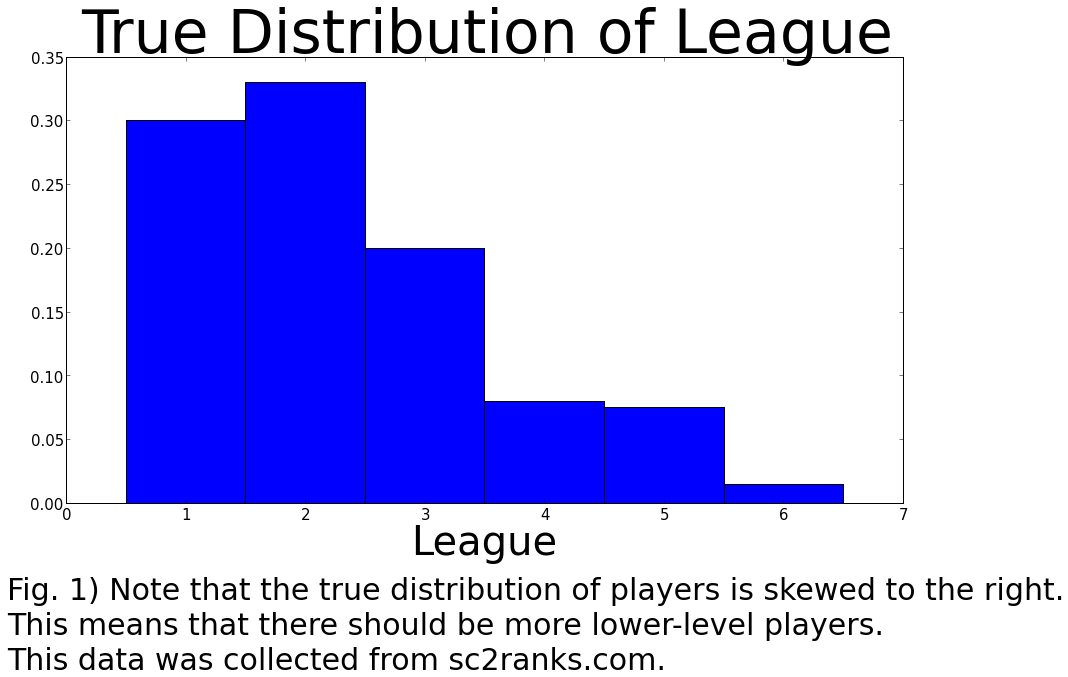
\includegraphics[max size={\textwidth}{\textheight}]{SC2Final_files/SC2Final_9_0.png}
    \par
    \end{center}
    
            \end{InvisibleVerbatim}
            
        
    
Our replays came from players who voluntarily submitted their games to
the forum. This means that our data is not a simple random sample. The
types of players who frequent a forum and would also be willing to
donate a replay are probably not representative of the player
population. This is seen quite clearly in these histograms of the
distribution of our data versus the distribution of the population. Our
data is biased towards having many more players in the higher leagues
because those players are the types that would be more willing to send
in their games. This means that we have to deal with a biased sample and
make sure to use models that will not be heavily influenced by this. Any
model that requires the probabilities of being in a certain class would
probably fail due to our data being so heavily skewed.

    

        % If the first block is an image, minipage the image.  Else
        % request a certain amount of space for the input text.
        \needspace{4\baselineskip}
        
        

            % Add document contents.
            
                \begin{InvisibleVerbatim}
                \vspace{-0.5\baselineskip}
    \begin{center}
    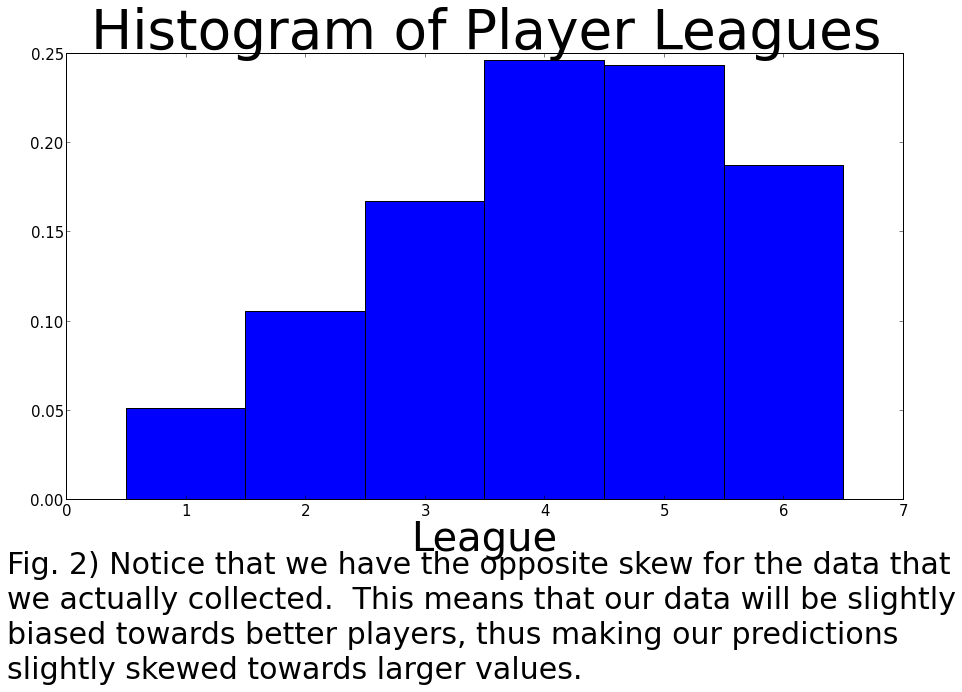
\includegraphics[max size={\textwidth}{\textheight}]{SC2Final_files/SC2Final_11_0.png}
    \par
    \end{center}
    
            \end{InvisibleVerbatim}
            
        
    
\part{Variables Used}The software that was used to process the game replays did so by
discretizing them into screenshots which were then used to count game
actions. Most variables in the dataset are just averages of those
actions over all screenshots. These screenshots are referred to as
Perception Action Cycles (PAC). These PAC's refer to when a player is
currently viewing some part of the map, so a single PAC is the player's
current view. If the player starts to view somewhere else in the game
that would be considered a new PAC. That gives rise to some more
variables like how often do they change their PAC, and how long does it
take for players to make their first action once they are in a new PAC.

If you look at the game screenshot below, take note of the bottom left
of the image. That image is called a minimap. In terms of sports, it
would be considered as the entire field of play. The point of dividing
things into different screenshots is that in this game you cannot
actually view the entire field at once. You can only view small sections
of the field, so the idea is that we want to know what kinds of things a
player is doing while viewing a certain part of the playing field.

    

        % If the first block is an image, minipage the image.  Else
        % request a certain amount of space for the input text.
        \needspace{4\baselineskip}
        
        

            % Add document contents.
            
                \makebox[0.1\linewidth]{\smaller\hfill\tt\color{nbframe-out-prompt}Out\hspace{4pt}{[}33{]}:\hspace{4pt}}\\*
                \vspace{-2.55\baselineskip}\begin{InvisibleVerbatim}
                \vspace{-0.5\baselineskip}
    \begin{center}
    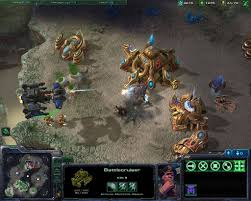
\includegraphics[max size={\textwidth}{\textheight}]{SC2Final_files/SC2Final_14_0.jpeg}
    \par
    \end{center}
    
            \end{InvisibleVerbatim}
            
        
    
Another important definition to understand is something called a hotkey.
Hotkeys are used by assigning a certain keyboard key to perform an
in-game action. The in-game actions can range from selecting a groups of
units, having those units move to a location, having them attack
something, having them perform a special attack, and so on. The idea is
that it is much faster to automatically select a group and then tell
them to do something with two key presses rather than having to find
them on the map, select them all with your mouse, then clicking the
button that refers to that action. We believe that a player's use of
hotkeys should do well at determining skill and thus a few of the
variables used are directly related to how a player handles hotkey
usage. In terms of the image above, note the bottom right portion of the
screen. That shows you all the actions that the selected unit can take.
When actually playing the game, the time it would take for you to find
your unit on the map and then click the button for the correct action is
precious time that can be saved using hotkeys. In a game where speed
counts, every little advantage you can get on your opponent should lead
to more wins.

Here is a list of all the variables created for this data set:

\begin{enumerate}[1.]
\item
  GameID: Unique ID number for each game (integer)
\item
  LeagueIndex: Bronze, Silver, Gold, Platinum, Diamond, Master,
  GrandMaster, and Professional leagues coded 1-8 (Ordinal)\\This is our
  response variable. It is an ordered variable that attempts to predict
  how skilled you are right now.
\item
  Age: Age of each player (integer)\\We are curious if certain age
  groups are better players than other groups. It is widely believed
  that older players tend to perform worse than younger players.
\item
  HoursPerWeek: Reported hours spent playing per week (integer)\\A
  possible measure of how dedicated the player is to improving.
\item
  TotalHours: Reported total hours spent playing (integer)\\A measure of
  how much experience a player has playing StarCraft 2.
\item
  APM: Action per minute (continuous)\\Average number of actions you
  make throughout the game. Many players believe this is the only or
  best measure of skill.
\item
  SelectByHotkeys: Number of unit or building selections made using
  hotkeys per timestamp (continuous)\\
\item
  AssignToHotkeys: Number of units or buildings assigned to hotkeys per
  timestamp (continuous)\\
\item
  UniqueHotkeys: Number of unique hotkeys used per timestamp
  (continuous)\\We believe the more you use hotkeys the more skilled you
  are as a player.
\item
  MinimapAttacks: Number of attack actions on minimap per timestamp
  (continuous)\\
\item
  MinimapRightClicks: number of right-clicks on minimap per timestamp
  (continuous)\\The use of the minimap is an alternative to moving your
  entire view. It requires some amount of foresight to use properly.
\item
  NumberOfPACs: Number of PACs per timestamp (continuous)\\
\item
  GapBetweenPACs: Mean duration in milliseconds between PACs
  (continuous)\\These two are related to map awareness. The more the
  player scouts the more information the player has about his opponent.
\item
  ActionLatency: Mean latency from the onset of a PACs to their first
  action in milliseconds (continuous)\\A measure of reflex time. It may
  also signify how much the player has planned ahead of time.
\item
  ActionsInPAC: Mean number of actions within each PAC (continuous)\\The
  higher this variable is, the more likely the player is just looking at
  one particular area of the map.
\item
  TotalMapExplored: The number of 24x24 game coordinate grids viewed by
  the player per timestamp (continuous)\\A measure of map awareness. It
  is generally believed that scouting provides useful information about
  the opponent.
\item
  WorkersMade: Number of SCVs, drones, and probes trained per timestamp
  (continuous)\\Vital for establishing a strong economy. Strong
  economies tend to allow players to build stronger armies.
\item
  UniqueUnitsMade: Unique units made per timestamp (continuous)\\A
  measure of how diverse a player's army is. A more diverse army is
  harder to defeat but often requires more maintenence.
\item
  ComplexUnitsMade: Number of ghosts, infestors, and high templars
  trained per timestamp (continuous)\\
\item
  ComplexAbilitiesUsed: Abilities requiring specific targeting
  instructions used per timestamp (continuous)\\When used properly,
  complex units and spells may provide additional advantages over the
  opponent.
\end{enumerate}\part{Trees}We attempted to address variable selection by utilizing decision trees.
Through some preliminary exploratory analysis we discovered that skills
which differentiate players of two particular leagues may not be the
same skills that differentiate players of two other leagues.
Intuitively, this happens because players of the lower leagues are at a
different stage of learning the game versus players of the higher
leagues. Because of this, we made the decision to focus on every
combination of two leagues rather than looking at everybody at once. For
each combination (referred to as a `matchup' from here on out), we
created a classification tree. The idea behind this choice is that by
looking at each matchup individually, perhaps we will find some trends
in the important variables that are used in separating the players in
each league. Then we will take some aggregate of those variables and use
them in our classification method.

We used 10-fold Cross Validation to find two optimal parameters: the
minimum number of samples required to split an internal node and the
minimum number of samples required to be at a leaf node. We used a zero
one loss function to evaluate each pair of parameter values.

We will now take a look at the trees of four particular matchups to get
a sense of which variables the trees are utilizing.  This first tree represents the comparison of the two lowest leagues.

    

        % If the first block is an image, minipage the image.  Else
        % request a certain amount of space for the input text.
        \needspace{4\baselineskip}
        
        

            % Add document contents.
            
                \makebox[0.1\linewidth]{\smaller\hfill\tt\color{nbframe-out-prompt}Out\hspace{4pt}{[}23{]}:\hspace{4pt}}\\*
                \vspace{-2.55\baselineskip}\begin{InvisibleVerbatim}
                \vspace{-0.5\baselineskip}
    \begin{center}
    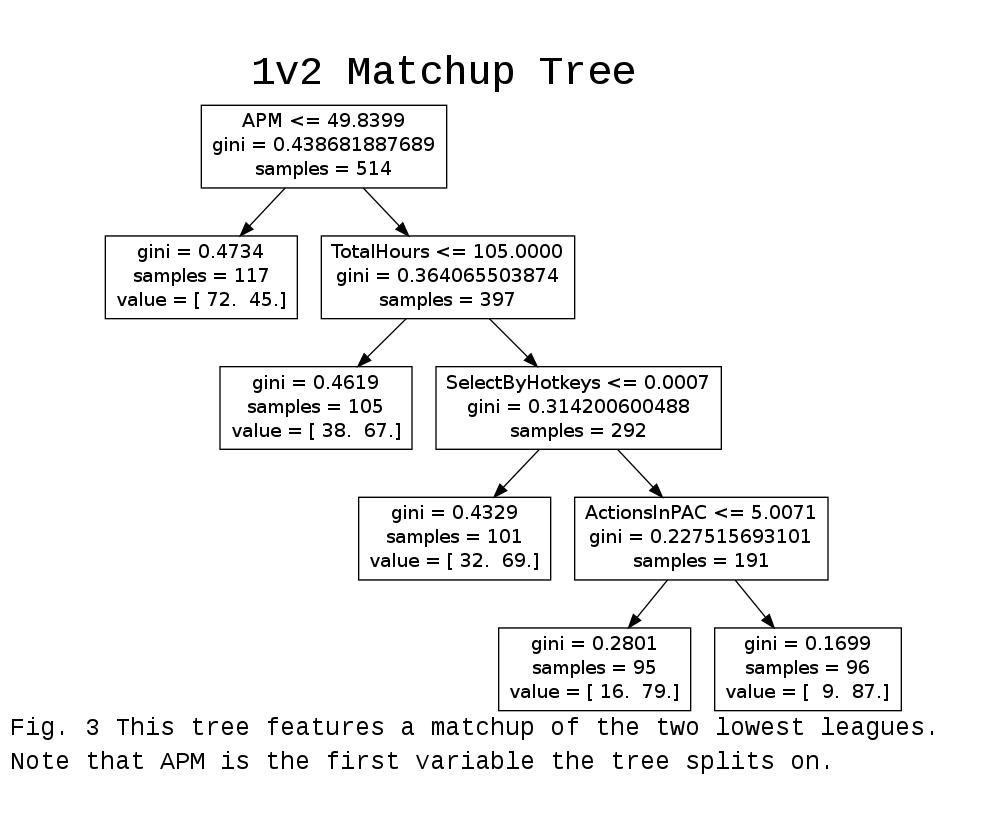
\includegraphics[max size={\textwidth}{\textheight}]{SC2Final_files/SC2Final_22_0.png}
    \par
    \end{center}
    
            \end{InvisibleVerbatim}
            
        
    
The first thing to notice is that APM is the first variable that the
tree splits on. APM, or Actions Per Minute, is the average number of
actions a player makes per minute. In other words, APM measures how
quickly you move and make actions throughout the game. Further down the
tree, notice the value for SelectByHotkeys is really small. This
suggests that if you select something using a hotkey even once you are
more likely to be in the higher league, thus matching our intuition that
using hotkeys is related to player skill.
\newpage
This next tree represents the comparison of a low league and a middle
league.

    

        % If the first block is an image, minipage the image.  Else
        % request a certain amount of space for the input text.
        \needspace{4\baselineskip}
        
        

            % Add document contents.
            
                \makebox[0.1\linewidth]{\smaller\hfill\tt\color{nbframe-out-prompt}Out\hspace{4pt}{[}22{]}:\hspace{4pt}}\\*
                \vspace{-2.55\baselineskip}\begin{InvisibleVerbatim}
                \vspace{-0.5\baselineskip}
    \begin{center}
    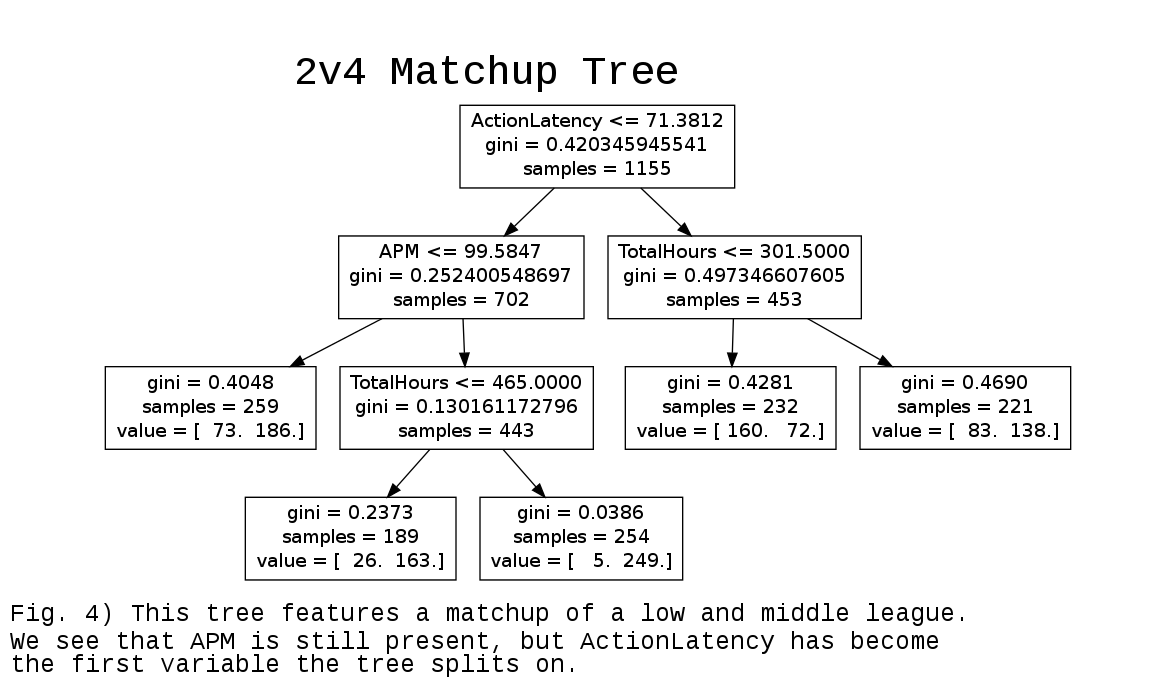
\includegraphics[max size={\textwidth}{\textheight}]{SC2Final_files/SC2Final_24_0.png}
    \par
    \end{center}
    
            \end{InvisibleVerbatim}
            
        
    
We see that APM is still present in the tree, but it is no longer the
first variable the tree splits on. Rather, the tree splits on
ActionLatency first. ActionLatency refers to the time it takes from
starting a new PAC to making an action. Furthermore, the tree consists
of only three variables and two of them are measures of game mechanics.
ActionLatency and APM combined with TotalHours suggest that the
difference between these two leagues is sheer amount of practice.
\newpage
This next tree represents the comparison of a middle league and a high
league.

    

        % If the first block is an image, minipage the image.  Else
        % request a certain amount of space for the input text.
        \needspace{4\baselineskip}
        
        

            % Add document contents.
            
                \makebox[0.1\linewidth]{\smaller\hfill\tt\color{nbframe-out-prompt}Out\hspace{4pt}{[}21{]}:\hspace{4pt}}\\*
                \vspace{-2.55\baselineskip}\begin{InvisibleVerbatim}
                \vspace{-0.5\baselineskip}
    \begin{center}
    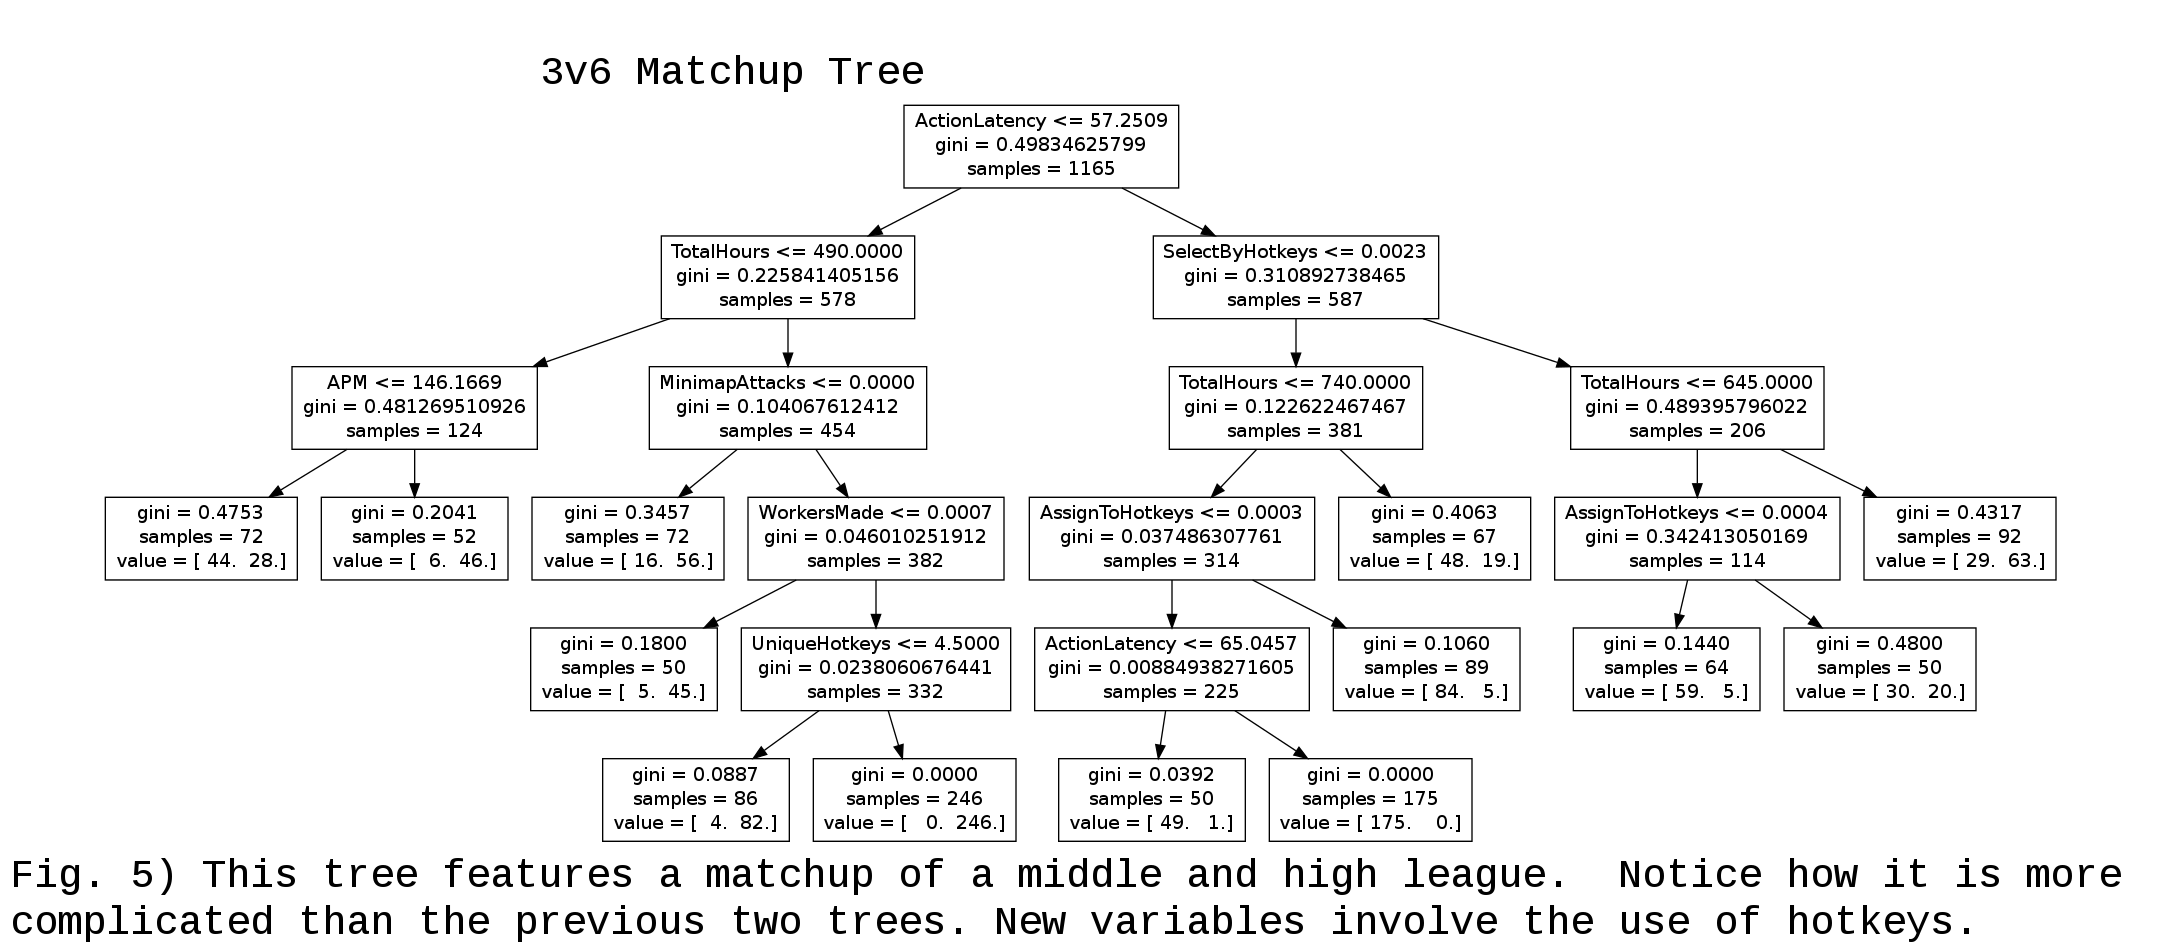
\includegraphics[max size={\textwidth}{\textheight}]{SC2Final_files/SC2Final_26_0.png}
    \par
    \end{center}
    
            \end{InvisibleVerbatim}
            
        
    
ActionLatency is the first variable the tree splits on, like the
previous tree. The most notable thing about this particular tree is the
amount of splits required to get a decent separation. The complexity of
the tree represents the difficulty our variables have in quantifying the
difference between medium players and good players. From personal
experience, medium level players tend to have similar if not the same
mechanical skills that high players have but they lack experience in
making decisions. This type of difference is not something that our
variables do a good job of taking into account, hence why there are so
many required to separate the leagues. Notice that there are multiple
variables that concern the use of hotkeys that were not present in the
previous two trees. It suggests that higher level players are more
comfortable at using hotkeys and thus are more likely to queue more
complex sequences of actions.

For the final tree, we compare the two highest leagues.

    

        % If the first block is an image, minipage the image.  Else
        % request a certain amount of space for the input text.
        \needspace{4\baselineskip}
        
        

            % Add document contents.
            
                \makebox[0.1\linewidth]{\smaller\hfill\tt\color{nbframe-out-prompt}Out\hspace{4pt}{[}20{]}:\hspace{4pt}}\\*
                \vspace{-2.55\baselineskip}\begin{InvisibleVerbatim}
                \vspace{-0.5\baselineskip}
    \begin{center}
    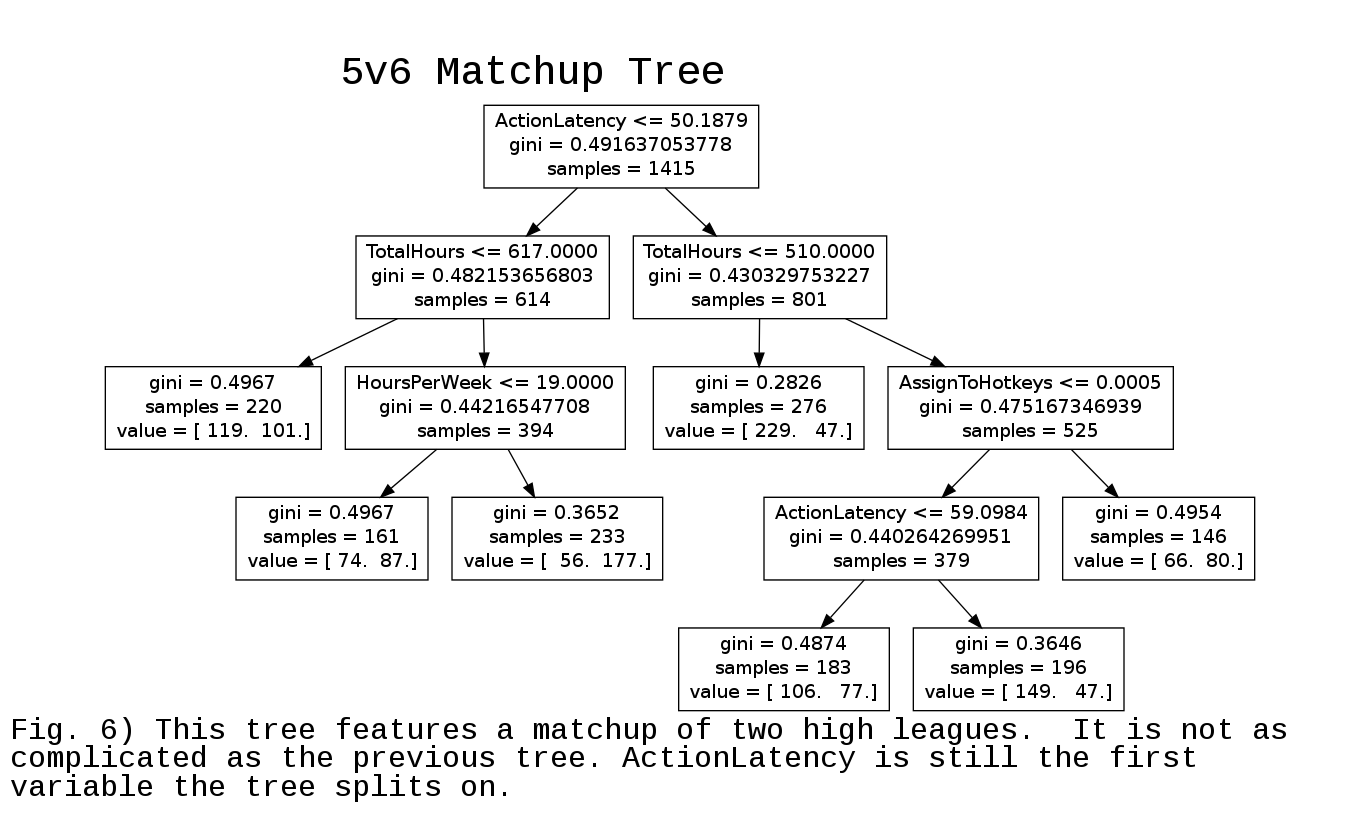
\includegraphics[max size={\textwidth}{\textheight}]{SC2Final_files/SC2Final_28_0.png}
    \par
    \end{center}
    
            \end{InvisibleVerbatim}
            
        
    
The tree is not as complicated as the previous one. ActionLatency
remains at the top, but note that TotalHours and HoursPerWeek are
present once again. What this suggests is that the biggest difference
between the two leagues is just experience and the amount of time
players put into the game. This makes sense because their skill levels
are quite similar mechanically, thus the differences come from smaller
details that are gained through playing the game more often.

To give the reader a summary of all the matchups, we created a table
that lists the three most important variable used by each of the trees.

    

        % If the first block is an image, minipage the image.  Else
        % request a certain amount of space for the input text.
        \needspace{4\baselineskip}
        
        

            % Add document contents.
            
                \begin{InvisibleVerbatim}
                \vspace{-0.5\baselineskip}
    \begin{center}
    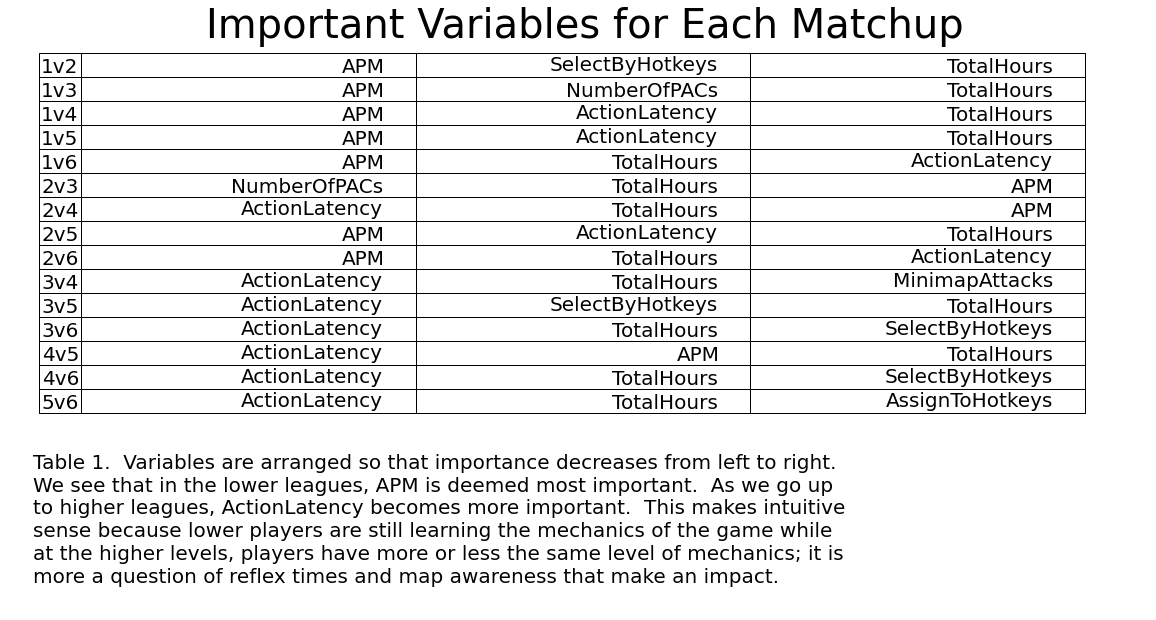
\includegraphics[max size={\textwidth}{\textheight}]{SC2Final_files/SC2Final_30_0.png}
    \par
    \end{center}
    
            \end{InvisibleVerbatim}
            
        
    
The table is structured so that importance decreases from left to right.
Notice that for all the matchups concerning the lowest league APM is the
most important variable. As we go up in leagues, ActionLatency becomes
more important. There is a clear shift in the trend of variables which
confirms our hypothesis that different matchups require different
variables to describe them.\part{K Nearest Neighbors}Now that we have an understanding of the variables that are important
for each of the leagues, we want to classify players into leagues using
these variables. We are looking to find a method that circumvents the
problems that the current ranking system has. For reference, the issues
that we have with the current ranking systems are threefold. First, it
requires too many games to give a reliable result. Second, players can
stop playing in order to protect their current ranking. And third, it is
hard to use ranking to compare your skill to players from previous times
due to inflation of points. Ideally, we would want a model that
addresses all 3 of these issues.

Since our dataset involves only a single game per person, if we can find
a method to classify that is at least fairly reliable then we have
addressed the first concern. The second and third concerns are due to
the way they use point values to keep track. So rather than grouping
players by point values, we should try to group them by skill level. We
want players of similar skill statistics to be classed into similar
leagues, thus the intuitive model choice here is K nearest neighbors
(KNN). This method is especially useful because it requires no
distributional assumptions and the effect of our biased sample is not
going to be so bad. Remember that our sample came from people who
volunteered their games, and we had a heavy bias towards higher leagues.
KNN does a fairly good job of not giving too biased of predictions even
with that kind of sample.

Now we want to get a sense of the way that KNN will behave for our
dataset. Since it is impossible to plot out all the variables used, we
decided to plot on ActionLatency and GapInPAC. GapInPAC is essentially
looking at how often a player moves the screen around to look at new
things while ActionLatency is how long it takes the player to do
something after moving the view to a new part of the map. Together they
should be at least somewhat representative of a player's multitasking
ability. Intuitively, better players will have smaller values for
GapInPAC and ActionLatency, meaning they are moving around a lot and
acting fast. We should expect then for this result to show up in the
following KNN decision plots.


    

        % If the first block is an image, minipage the image.  Else
        % request a certain amount of space for the input text.
        \needspace{4\baselineskip}
        
        

            % Add document contents.
            
                \begin{InvisibleVerbatim}
                \vspace{-0.5\baselineskip}
    \begin{center}
    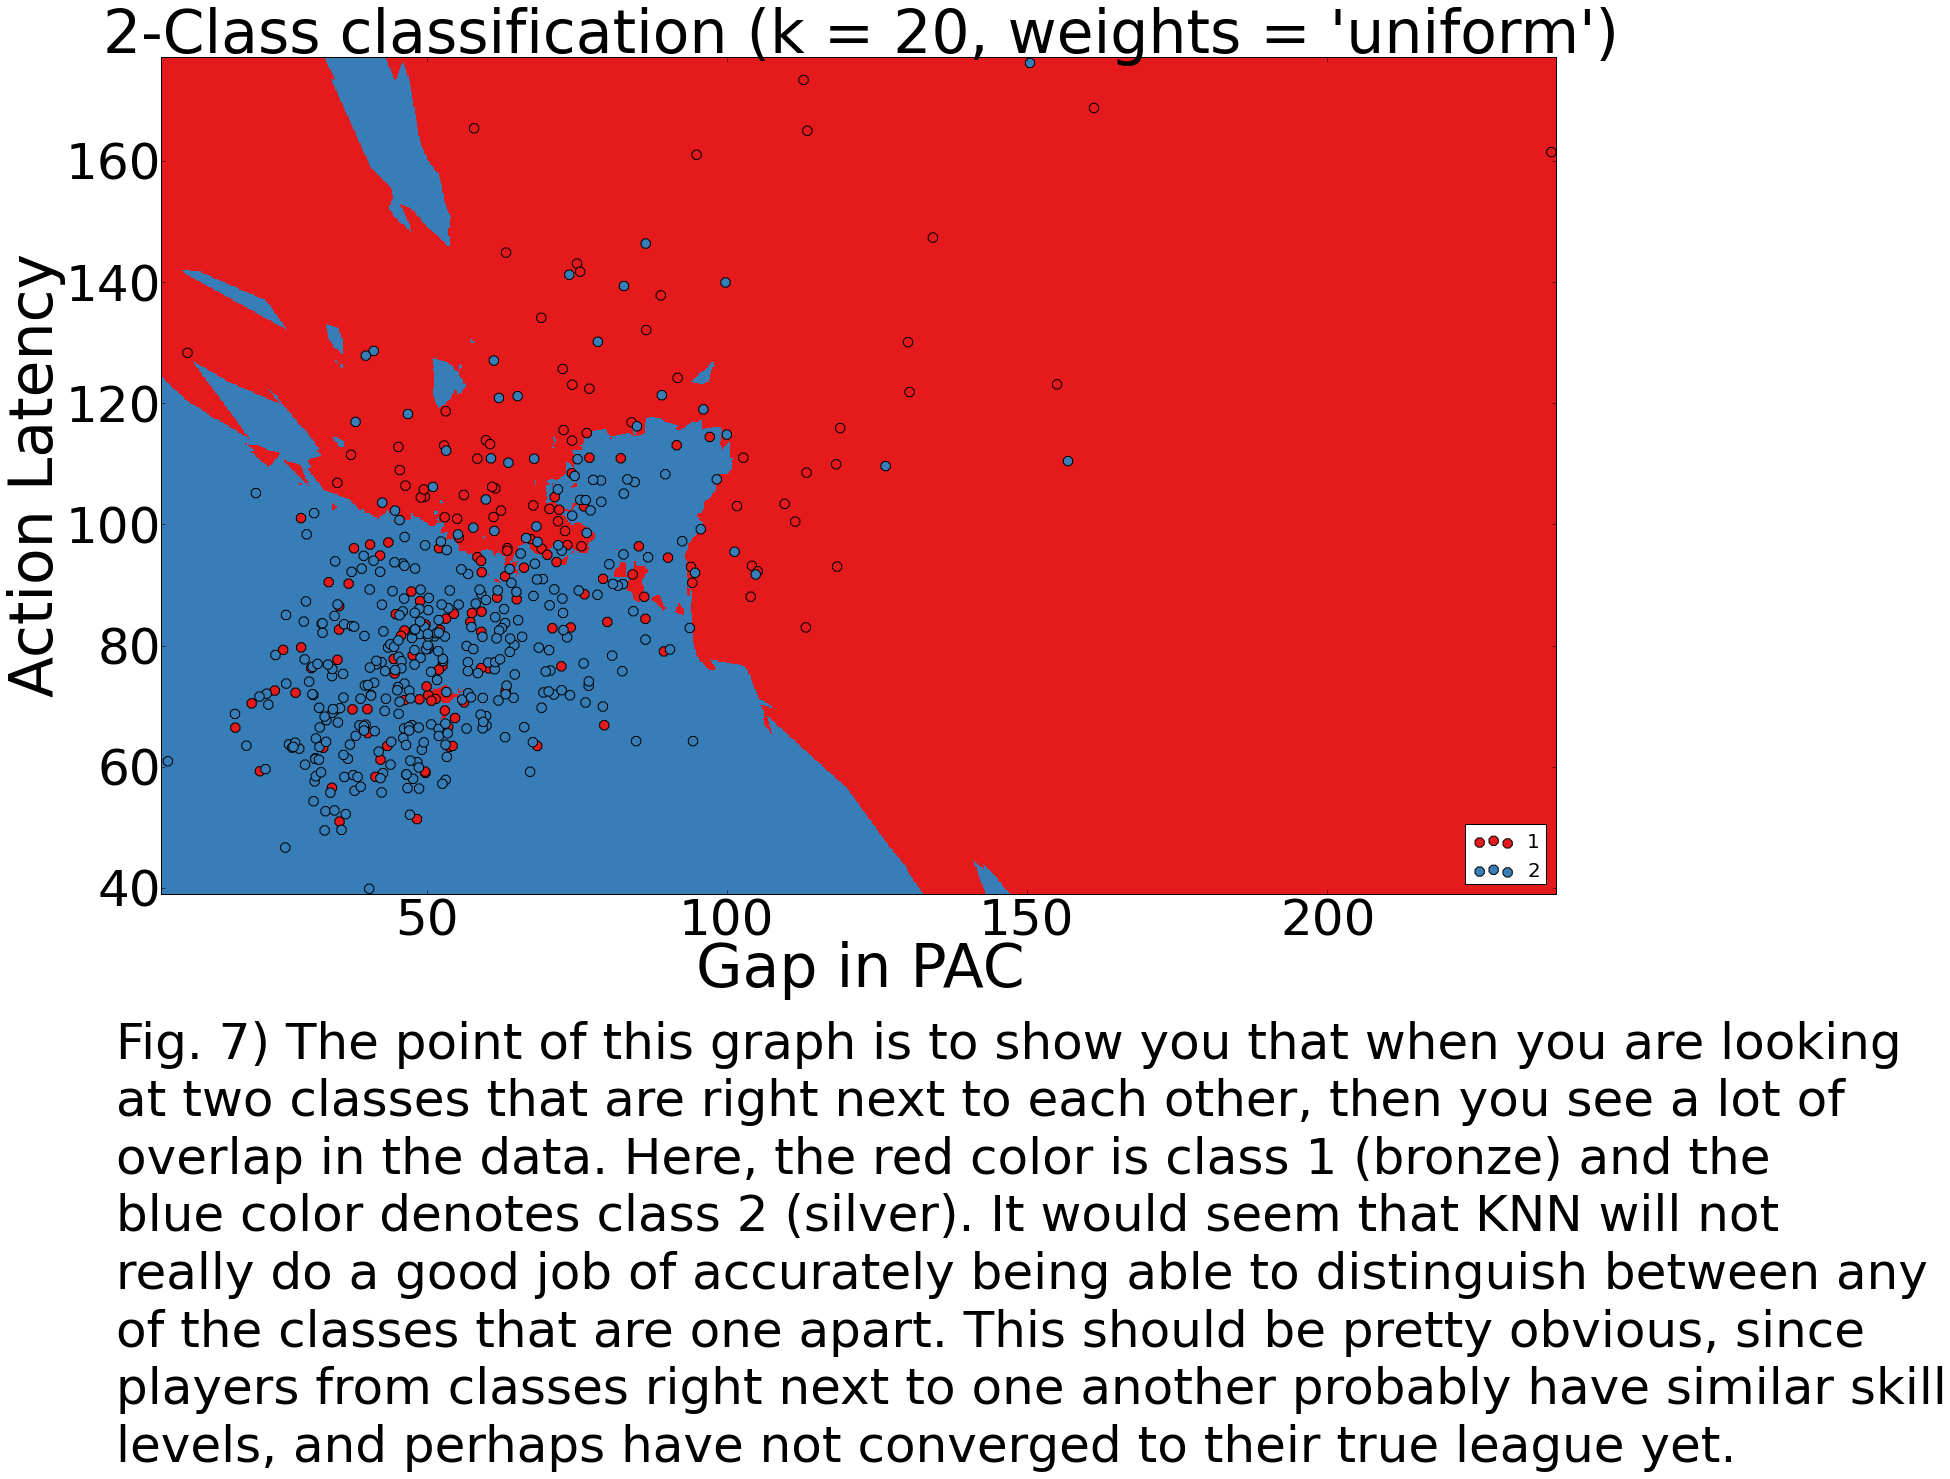
\includegraphics[max size={\textwidth}{\textheight}]{SC2Final_files/SC2Final_35_0.png}
    \par
    \end{center}
    
            \end{InvisibleVerbatim}
            
        
    
This plot uses a subset of the data containing only players from class 1
(the worst) and class 2 (second worst). As far as the boundaries go, it
follows our intuition that the better league is the one closer to the
origin (smaller values for both variables). However, when it comes to
leagues that are right next to each other it seems like there is a very
large overlap of the players. This means that players who are in leagues
one off from another (i.e.~leagues 1 and 2) tend to have similar skill
statistics. In terms of ranking, this could be due to the fact that they
are not yet in their `true' league because they haven't played enough
games to get there. So our belief then is that the KNN model is grouping
people on their current skill which does a better job of predicting
their true skill than their wins and losses. As long as our variables
are representative of a player's skill, then this model is doing very
well.
\newpage
This next plot is made to contrast the one from before.

    

        % If the first block is an image, minipage the image.  Else
        % request a certain amount of space for the input text.
        \needspace{4\baselineskip}
        
        

            % Add document contents.
            
                \begin{InvisibleVerbatim}
                \vspace{-0.5\baselineskip}
    \begin{center}
    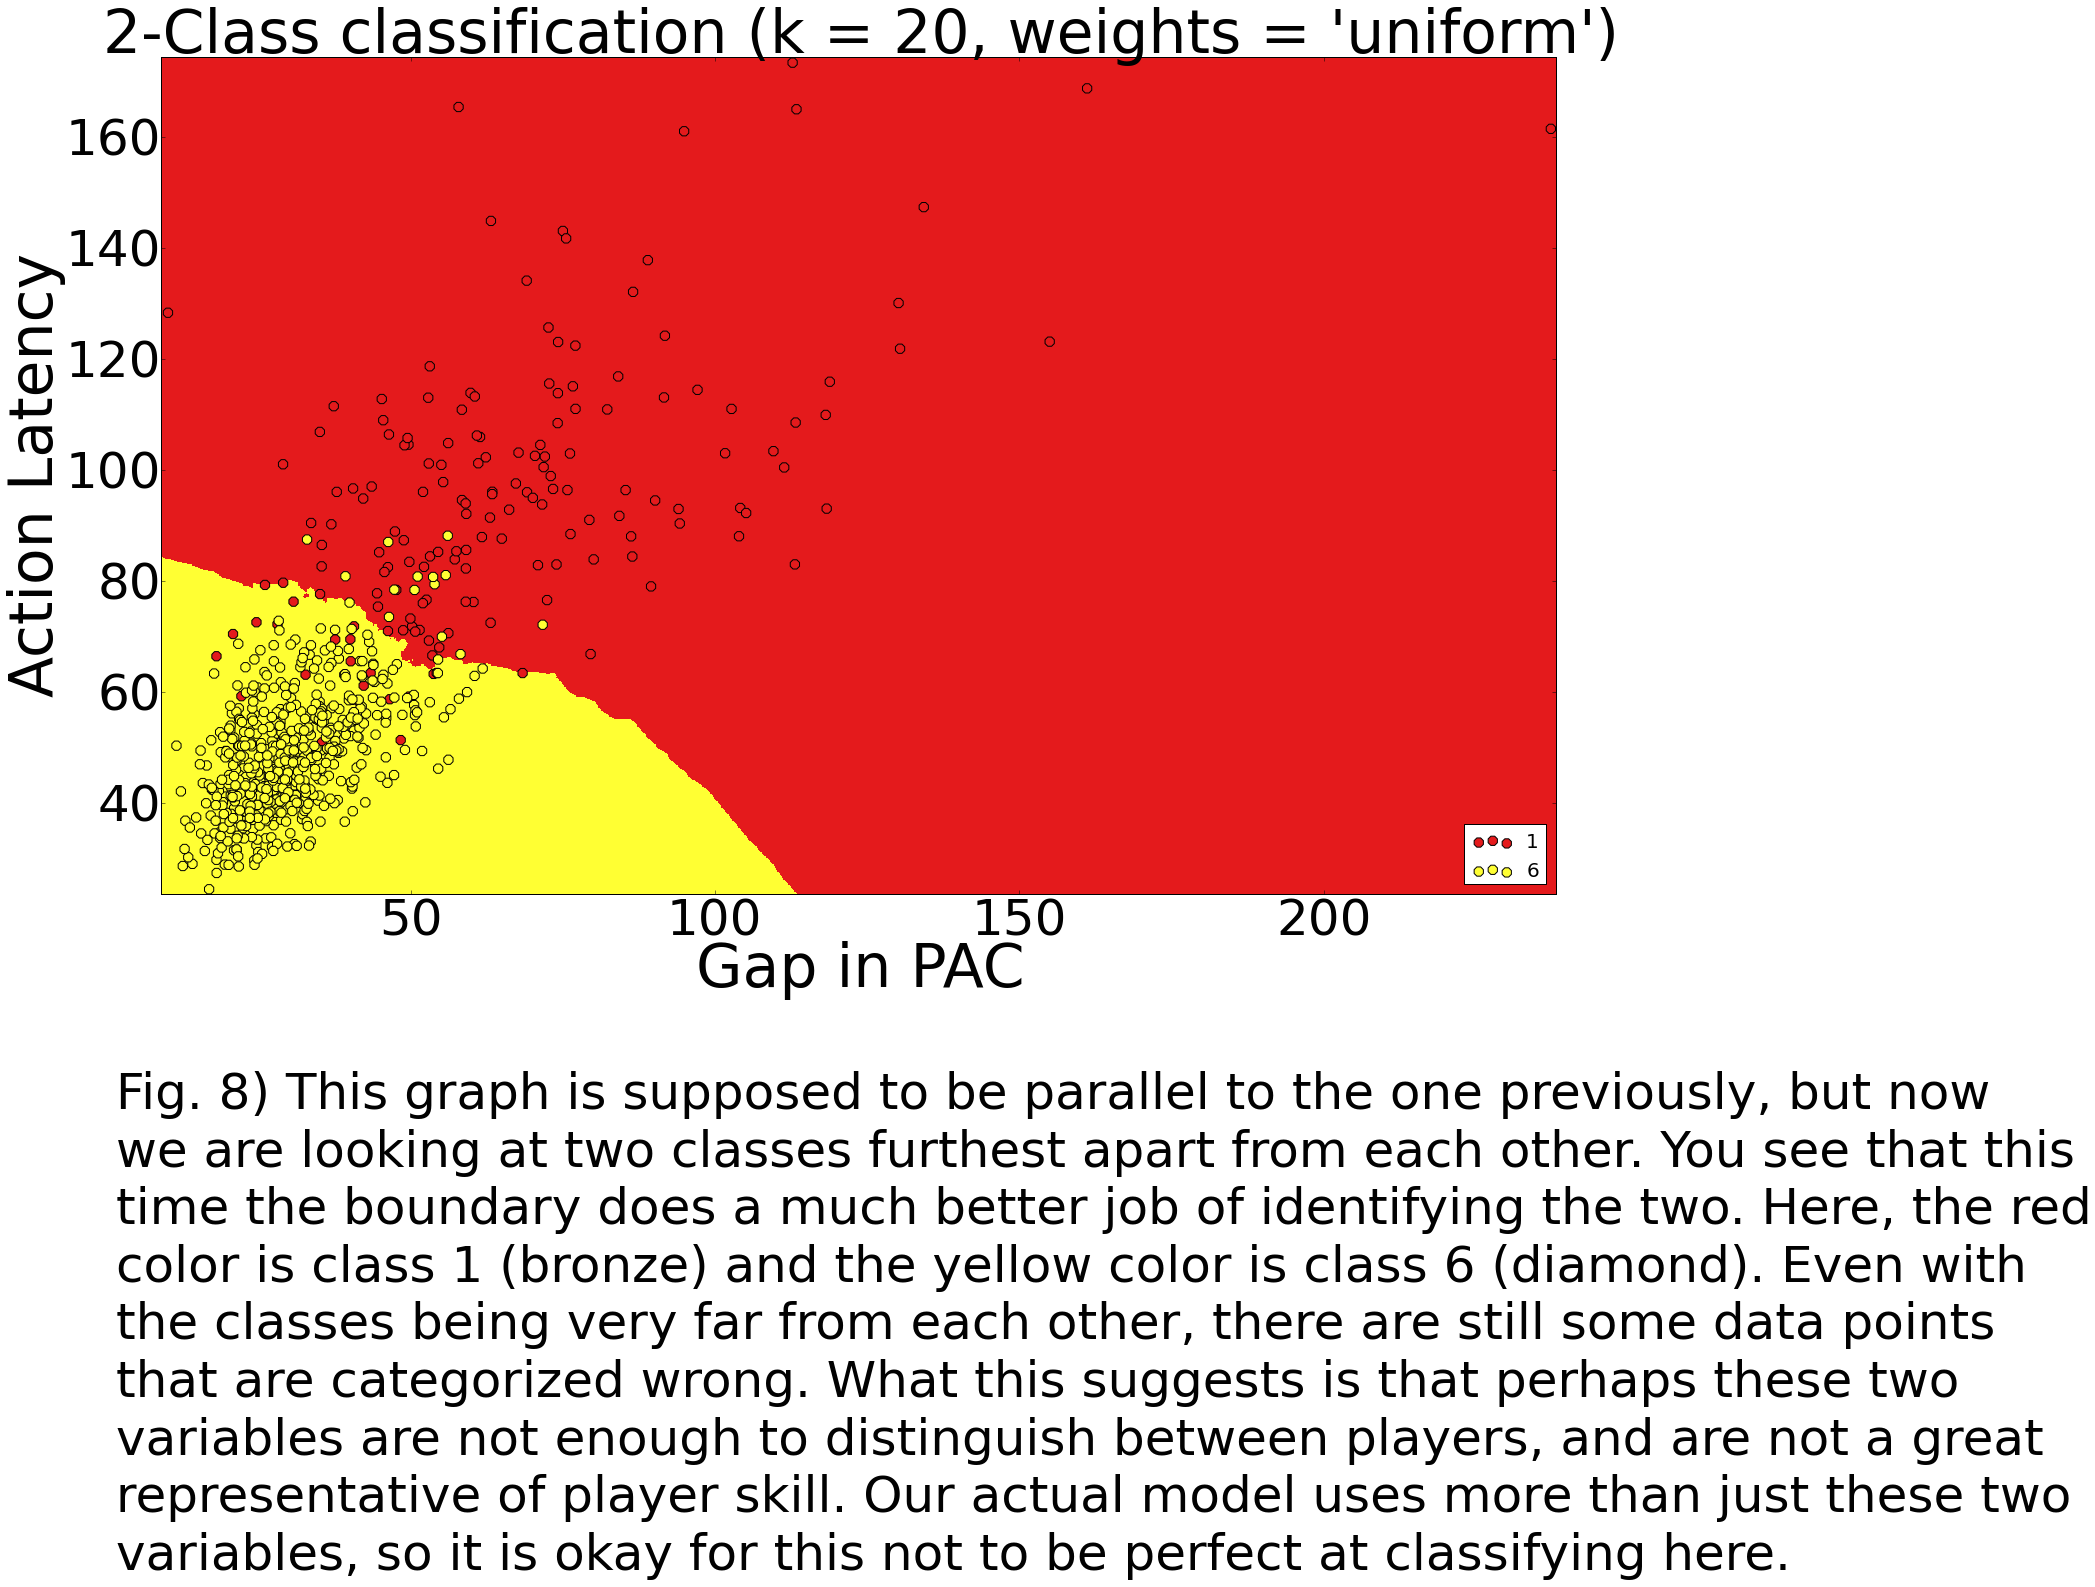
\includegraphics[max size={\textwidth}{\textheight}]{SC2Final_files/SC2Final_37_0.png}
    \par
    \end{center}
    
            \end{InvisibleVerbatim}
            
        
    
This one contains only players from class 1 and class 6, which are on
the opposite sides of the skill spectrum. Notice here that the
separation is much more clearly defined and there is a lot less
misclassification. This is to be expected because even if the current
ranking system is not so good, it is not extremely off. Saying that
someone currently in league 1 is actually playing at a league 6 level is
a pretty huge statement. Luckily this does not seem to happen too often
so our model is not completely contradicting the current ranking, which
is good. Theoretically, we should expect to see that the full KNN model
should have many similar predictions and many slight differences, but
not too many large contradictions with the current rankings.\part{Building the Model}Now we fit a KNN model by cross validating over K, using the zero-one
loss function. We used the variable selection done in the first section
and selected the following 5 variables:

\begin{enumerate}[1.]
\item
  TotalHours: Reported total hours spent playing (integer)
\item
  APM: Action per minute (continuous)
\item
  AssignToHotkeys: Number of units or buildings assigned to hotkeys per
  timestamp (continuous)
\item
  MinimapAttacks: Number of attack actions on minimap per timestamp
  (continuous)
\item
  ActionLatency: Mean latency from the onset of a PACs to their first
  action in milliseconds (continuous)
\end{enumerate}


This is the confusion matrix that compares our predicted league versus
the player's current league.

    

        % If the first block is an image, minipage the image.  Else
        % request a certain amount of space for the input text.
        \needspace{4\baselineskip}
        
        

            % Add document contents.
            
                \begin{InvisibleVerbatim}
                \vspace{-0.5\baselineskip}
    \begin{center}
    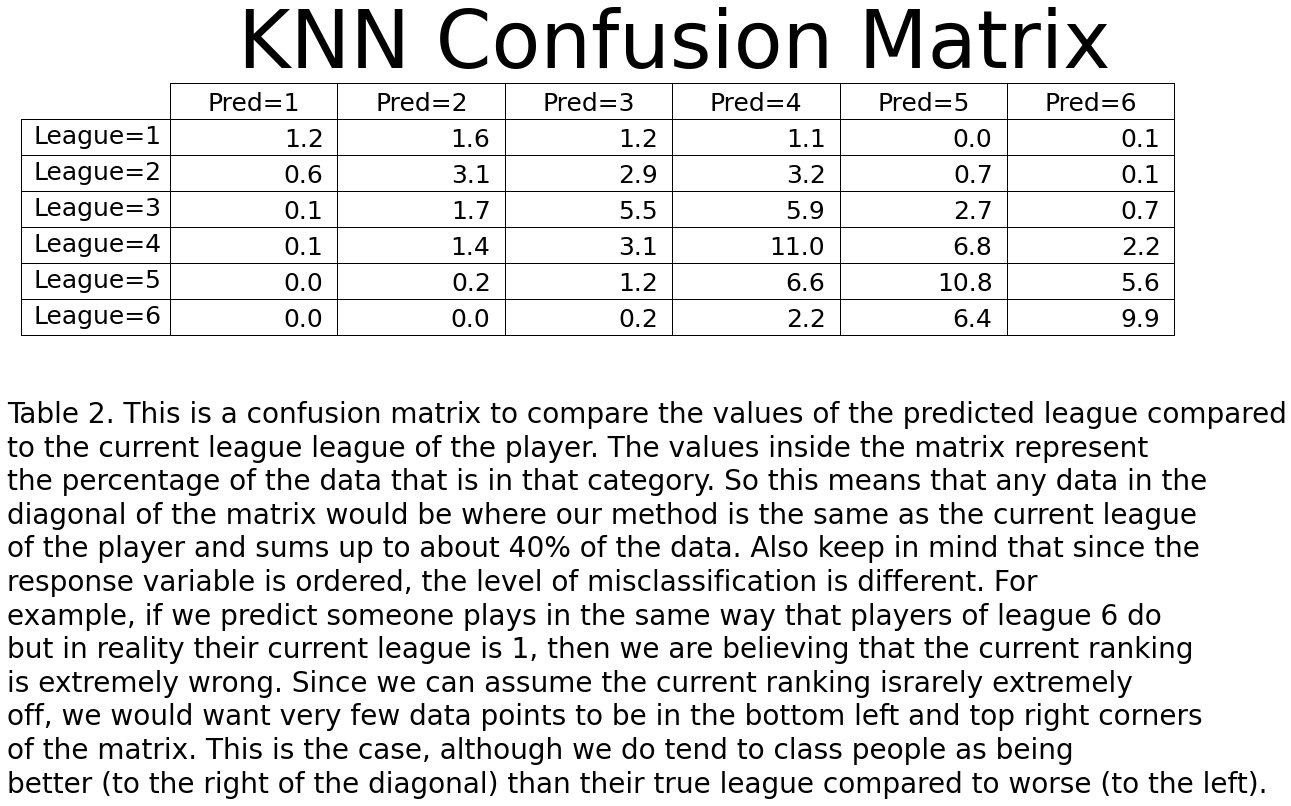
\includegraphics[max size={\textwidth}{\textheight}]{SC2Final_files/SC2Final_45_0.png}
    \par
    \end{center}
    
            \end{InvisibleVerbatim}
            
        
    
The values inside the matrix are the percent of players in that
particular cell. The variable on the top is our predicted league using
KNN, and the variable on the left is the current league. That means that
any data that falls along the diagonal of the confusion matrix is when
our model is in agreement with the current rank. This sums up to 40\% of
our data that we consider to be in the correct league at the moment.

Since our data is ordered, the level of difference between predicted
value and current rank is different. If someone is currently rank 6 and
we think they are playing at the same level as rank 1 players, then we
are stating that the current ranking system is immensely inadequate at
predicting skill. So in reference to the matrix, this means any data in
the upper right and lower left corners signifies a very large difference
in what we predict versus current ranking. We said previously that we
expect for this to happen very rarely, which is indeed the case if you
check the values: 80\% of the data lies either on the diagonal or
directly off the diagonal.\part{Conclusion}We found several interesting absences of variables from the matchups.
For starters, Age was never one of the top three variables for any tree
to split on. Typically, the belief is that older players have slower
reflexes which would put them at a disadvantage but this did not show up
prominently. None of the in-game variables (i.e.~WorkersMade,
UniqueUnitsMade, etc.) showed up as well, signifying that there is no
optimal strategy that leads to becoming a better player. Flipping it
around, we were surprised to see TotalHours show up in many of the
matchups. This is actually a bad thing because time is not a measure of
the quality of play: a player may spend many hours playing horribly but
our model would assume the opposite, that the player spent many hours
playing very well.

If we were to improve the study, we would want to try and find a more
random sample. In particular we would like a sample that reflects the
current league distribution, so we would want more lower league players
and less higher league players. In addition, we would want to try more
advanced methods such as random forests and support vector machines
although those methods would lack interpretability.

In conclusion, defining skills are heavily based on context; there is no
one variable that can be used well in every matchup. For matchups
involving lower league players, APM is very important. As the leagues go
up, ActionLatency becomes more important. Our KNN model does a good job
at predicting the true league of a player while maintaining a simple and
intuitive interpretation. Players may now parse their own replays and
send the output through our KNN model to see which league matches their
current skills. We have successfully created a method of predicting
player skill that does not have the problems that the current ranking
system has.\part{References}Mark Blair, Joe Thompson, Andrew Henrey, Bill Chen. `SkillCraft1 Master
Table Dataset Data Set'.
http://archive.ics.uci.edu/ml/datasets/SkillCraft1+Master+Table+Dataset\#.

`Scikit-learn: Machine Learning in Python', Pedregosa et al., JMLR 12,
pp.~2825-2830, 2011.
        

        \renewcommand{\indexname}{Index}
        \printindex

    % End of document
    \end{document}


